% TODO:
%   - 添加封面

\documentclass[UTF8,12pt,a4paper]{ctexart}
\ctexset { section = { format={ \Large \bfseries } } }
\ctexset{ bibname = \leftline{参考资料} }

\usepackage{graphicx}
\usepackage{geometry}
\usepackage{multirow}
\usepackage{booktabs}
\usepackage{enumerate}
\usepackage{array, caption, threeparttable}
\usepackage{float}
\usepackage{amsmath}
\usepackage[colorlinks,linkcolor=blue]{hyperref}
\usepackage{listings}
\usepackage{color}

\geometry{left=2.5cm, right=2.5cm, top=3.0cm, bottom=3.0cm}

\definecolor{dkgreen}{rgb}{0,0.6,0}
\definecolor{gray}{rgb}{0.5,0.5,0.5}
\definecolor{mauve}{rgb}{0.58,0,0.82}
\lstset{frame=tb,
  language=Python,
  aboveskip=3mm,
  belowskip=3mm,
  showstringspaces=false,
  columns=flexible,
  basicstyle={\scriptsize\ttfamily},
  keywordstyle=\color{blue},
  commentstyle=\color{dkgreen},
  stringstyle=\color{mauve},
  breaklines=true,
  breakatwhitespace=true,
  tabsize=2
}


\title{软件需求分析、架构的4+1视图模型和可信性分析研究——以Yagmail邮件发送系统为例}
\author{卓旭(212138)~李竞宇(212115)~李文炜(212079)}
\date{2021年11月}

\begin{document}

\maketitle

    \begin{abstract}
        Yagmail \cite{yagmail} 是一个用于进行邮件发送的软件系统,使用Python语言编写且开源。
        其调用方式简单,功能齐全,结果可靠,被许多需要邮件发送功能
        的Python应用所集成。“邮件发送”对软件可信性的要求很高,
        如邮件内容格式要正确保留、发送成功率要高、等等。本文
        以一个略经修改的Yagmail的Fork为例,进行需求分析,研究软件架构。
        进一步地,从多方面探究软件架构对软件可信性的影响,并给出相关实验结果,
        佐证提出的论证。本文的所有相关代码均可在 \url{github.com/z0gSh1u/sa-analysis}
        取得。
    \end{abstract}

\newpage
\tableofcontents

\newpage
\section{Yagmail系统需求说明}
    \begin{figure}[H]
        \centering
        
\includegraphics[width=0.1\textwidth]{figure/yagmail-icon.png}
        \caption{Yagmail软件系统图标}
    \end{figure}

    首先简单介绍Yagmail的使用方式作为背景。在Yagmail的官方文档中,
    给出了核心功能:邮件发送的调用方式,具体如下。该示例代码首先认证了一个发件邮箱账号,
    然后组织邮件内容(允许文本、HTML富文本、附件),最后调用send方法,即可向收件人发送邮件。
    
    \begin{lstlisting}
    import yagmail
    yag = yagmail.SMTP('myUsername', 'myPassword')
    contents = ['This is the body, and here is just text http://somedomain/image.png',
                'You can find an audio file attached.', '/local/path/song.mp3']
    yag.send('to@someone.com', 'subject', contents)
    \end{lstlisting}

    本节接下来,我们将利用FURPS+模型\cite{furps}以及相关用例,对Yagmail系统的系统需求进行分析与说明。

\subsection{功能性(F)}

    本小节给出Yagmail使用过程中的两个常用用例:登录认证和邮件发送,并通过
    用例图进一步阐释了用例。

\textbf{用例1:登录认证}

\begin{table}[H]
\centering
\begin{tabular}{p{0.25\textwidth}|p{0.7\textwidth}}
\hline
\textbf{参与者及兴趣列表} & 由发件人启动。在安全,账户信息不泄露的前提下,简单快速的登录认证。                                                                      \\ \hline
\textbf{入口条件}     & 安装并导入Yagmail。                                                                                          \\ \hline
\textbf{出口条件}     & 发件人成功认证,Yagmail得到发件地址权限。                                                                               \\ \hline
\textbf{事件流}      & \begin{tabular}[c]{@{}l@{}}1. 发件人导入Yagmail包,并连接网络;\\ 2. 发件人调用register方法,填入发件地址和密码信息。\end{tabular}      \\ \hline
\textbf{扩展或替代流程}  & \begin{tabular}[c]{@{}l@{}}2a. 不使用密码,而使用Keyring认证;\\ 2b. 不使用密码,而使用OAuth认证。\end{tabular}                \\ \hline
\textbf{质量需求}     & \begin{tabular}[c]{@{}l@{}}1. 不受平台、操作系统的影响;\\ 2. 认证后安全保存信息,一段时间内不需要重复登录;\\ 3. 保证密码数据不被泄露。\end{tabular} \\ \hline
\end{tabular}
\end{table}

\textbf{用例2:发送邮件}

\begin{table}[H]
\centering
\begin{tabular}{p{0.25\textwidth}|p{0.7\textwidth}}
\hline
\textbf{参与者及兴趣列表} & 由发件人启动,希望邮件准确无误地发送给收件人。 收件人想要接收到内容无误的邮件。                                                                 \\ \hline
\textbf{入口条件}     & 发件人已成功认证并连接网络。                                                                                          \\ \hline
\textbf{出口条件}     & Yagmail成功发送邮件,收件人收到无误的邮件。                                                                               \\ \hline
\textbf{事件流}      & \begin{tabular}[c]{@{}l@{}}
1. 发件人构造SMTP对象,准备发件;\\ 
2. 发件人调用send方法,填入收件地址、主题、正文等信息;\\
3. 收件人成功接收到邮件。
\end{tabular}      \\ \hline
\textbf{扩展或替代流程}  & \begin{tabular}[c]{@{}l@{}}
2a. 主题可以为空;\\
2b. 正文可以为空;\\
2c. 邮件可以添加附件。\end{tabular}                \\ \hline
\textbf{质量需求}     & \begin{tabular}[c]{@{}l@{}}
1. 支持群发多个收件人;\\ 
2. 正文支持HTML富文本,图片,纯文本等格式;\\ 
3. 对非法输入有合理反馈。\end{tabular} \\ \hline
\end{tabular}
\end{table}

Yagmail的用例图如下图所示:

\begin{figure}[H]
    \centering
    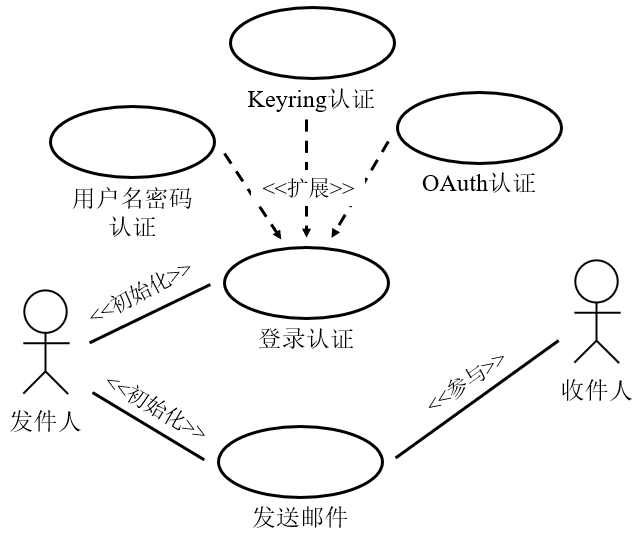
\includegraphics[width=0.6\textwidth]{figure/usecasediagram.png}
    \caption{Yagmail用例图}
\end{figure}

\subsection{可用性(U)}

在安装方面,Yagmail安装简单,只需使用Python自带的包管理工具pip,执行命令
pip install yagmail[all]即可安装。对于低版本的Python(如2.X版本),Yagmail
也提供了垫片代码(Polyfill)与回退方案(Fallback)以支持。

在文档方面,官方提供了详尽的使用文档,介绍了软件的使用细节,以及可能遇到的问题的解决方案与反馈途径。软件整体具有高可用性。

\subsection{可靠性(R)}

在执行失败率方面,根据Yagmail在其他软件系统中的集成使用的反馈,在正确调用的前提下,Yagmail的执行失败率低。

在可恢复性方面,Yagmail定义了一系列自定义异常,并对其他可能的异常也做了try-catch处理。因局部错误导致整个软件系统崩溃的可能性低,整体可恢复性较高。

在可预测性方面,Yagmail的代码结构简单,各模块间相互调用链路清晰。通过通读代码,判断Yagmail整体执行路径具有较好的可预测性,软件行为也随之具有较好的可预测性。

对于调用链路、执行成功率等方面的具体分析,将在第三节:可信性分析中具体阐述。

\subsection{性能(P)}

在软件系统的性能方面,在进行邮件发送等基础功能的使用时,Yagmail系统内部消耗的响应时间很短,这使得
Yagmail的吞吐量得以提升。另外,Yagmail库的大小仅约60KB,且依赖库基本都为Python的标准库,所以
在其他集成的软件系统中,资源占用率很低。

\subsection{可支持性(S)}

在可维护性方面,Yagmail可随时通过Python的包管理工具pip进行更新,相关错误问题可及时通过GitHub Issue与开发者联系,获得维护修改。

在国际化(i18n)方面,Yagmail自身支持邮件内容按UTF-8编码,在不同语言之间具有较好的国际化兼容性。

\subsection{其它(+)}

Yagmail的实现语言为Python,使用MIT License分发。流行、稳健的语言选型增强了Yagmail的稳定性,而
宽松的License选择使Yagmail被开源社区更广泛地使用与集成。

\newpage
\section{Yagmail架构的4+1视图模型}

    本节,我们应用Kruchten的对软件架构的“4+1”视图模型\cite{fourplusone},
    对Yagmail系统的架构进行了多角度分析。

\subsection{逻辑视图}
    逻辑视图通过使用类图和类模板,体现Yagmail系统的不同功能需求。Yagmail系统通过yagmail.SMTP与smtplib.SMTP的交互,建立起邮件构建与邮件发送的桥梁。yagmail.SMTP通过使用地址校验工具类,校验收件发件地址;通过smtplib.SMTP进行基于账户密码的验证、基于Keyring的认证,或OAuth认证,获得发件地址控制权;EmailBuilder构建邮件传递给yagmail.SMTP,经处理后交由smtplib.SMTP实际发送邮件到收件地址。Yagmail系统还通过基础设施类保存日志或者错误信息。
    
    Yagmail的逻辑视图示意图如下图所示:
    
    \begin{figure}[H]
        \centering
        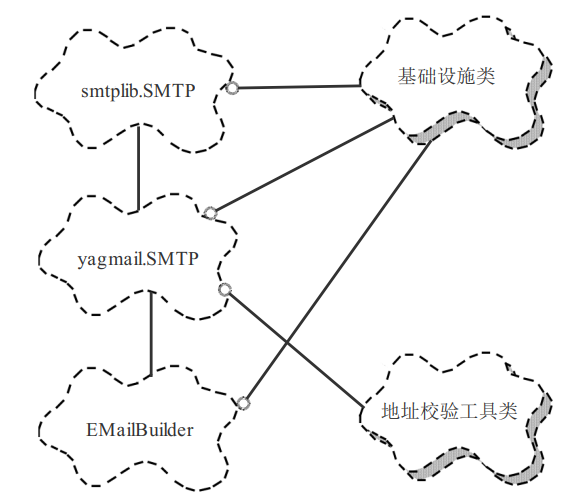
\includegraphics[width=0.55\textwidth]{figure/log-view.png}
        \caption{Yagmail逻辑视图}
        \label{fig:log-view}
    \end{figure}

\subsection{过程视图}
    过程视图给出了Yagmail系统使用时的几个主要任务,每个任务是一个独立的控制过程,可以在一个处理节点上独立单独调度,但每次原始调用产生的各过程之间需要串行执行,最终才能完成邮件发送。
    
    Yagmail的过程视图示意图如下图所示:
    
    \begin{figure}[H]
        \centering
        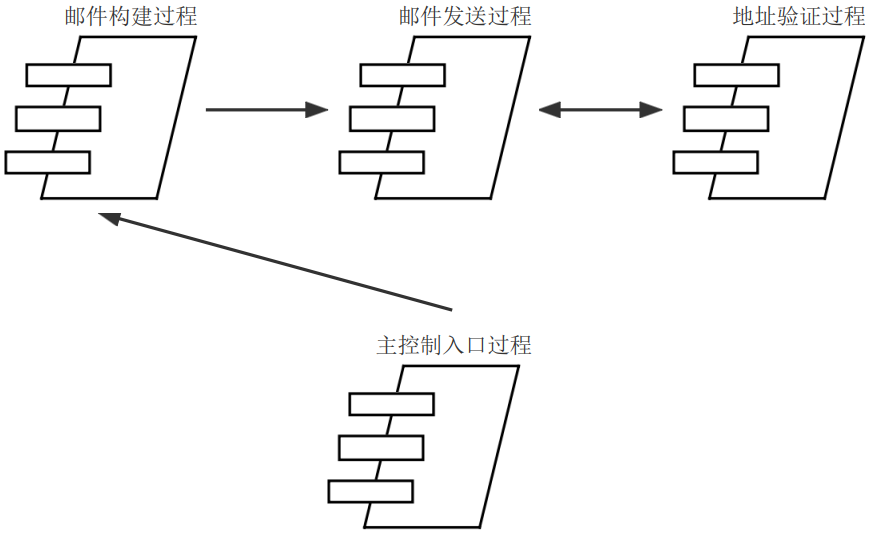
\includegraphics[width=0.65\textwidth]{figure/pro-view.png}
        \caption{Yagmail过程视图}
        \label{fig:pro-view}
    \end{figure}

\subsection{开发视图}

    开发视图给出了Yagmail软件系统各模块的静态组织结构。Yagmail的子系统层次可分为5层:日志、
    工具、错误模块工作在硬件、操作系统、Python解释器上,构成了基础设施子系统层次;地址校验
    模块进一步构成可靠收件地址验证子系统;账密验证、Keyring验证、OAuth验证模块进一步构成
    发件地址权限控制子系统;邮件构建模块进一步构成待发送邮件子系统;邮件发送模块进一步构成
    Yagmail邮件发送系统。
    
    Yagmail的开发视图示意图如下图所示:

    \begin{figure}[H]
        \centering
        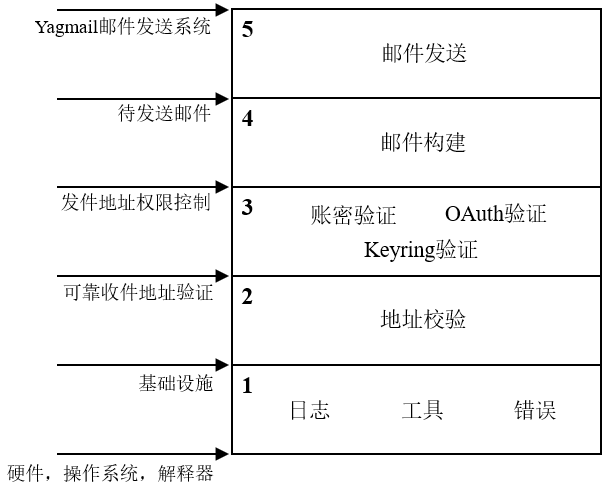
\includegraphics[width=0.7\textwidth]{figure/dev-view.png}
        \caption{Yagmail开发视图}
        \label{fig:dev-view}
    \end{figure}

\subsection{物理视图}

    物理视图考虑了Yagmail系统在运行的过程中,是如何将诸如网络过程、运算过程等各元素映射到
    具体的物理处理节点上进行运行的。
    
    考虑单机运行情况下的处理核心和作为外部设备的网卡,Yagmail系统的物理视图示意图如下图所示:
    
    \begin{figure}[H]
        \centering
        
\includegraphics[width=0.45\textwidth]{figure/phy-view.png}
        \caption{Yagmail物理视图}
        \label{fig:phy-view}
    \end{figure}

\subsection{场景}

    一个场景是一或多个用例的组合。
    通过场景的组织,可以展示上述四个视图中元素的协调工作模式。我们分析了Yagmail最重要的两个
    需求:发件地址权限的获取、邮件的发送,给出了对应的对象场景图。
    
    对于发件地址权限获取的场景,sender首先借助地址校验工具类对发件地址进行校验,然后
    凭地址与登录凭证与smtp沟通,从而最终取得对发件地址的发件权限的控制权。
    \begin{figure}[H]
        \centering
        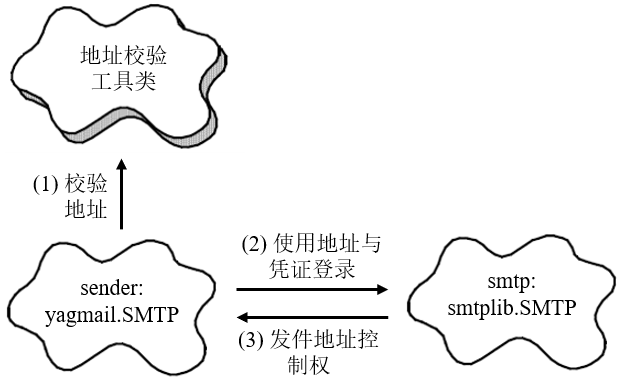
\includegraphics[width=0.65\textwidth]{figure/scene-1.png}
        \caption{Yagmail场景1:发件地址权限的获取}
        \label{fig:scene-1}
    \end{figure}
    
    对于邮件的发送的场景,带有发件地址控制权的参数化的sender首先与builder合作,完成邮件内容的构建。
    然后,向smtp发起发送邮件的请求。smtp回传发送邮件的结果,并产生一封邮件(如果成功)。
    \begin{figure}[H]
        \centering
        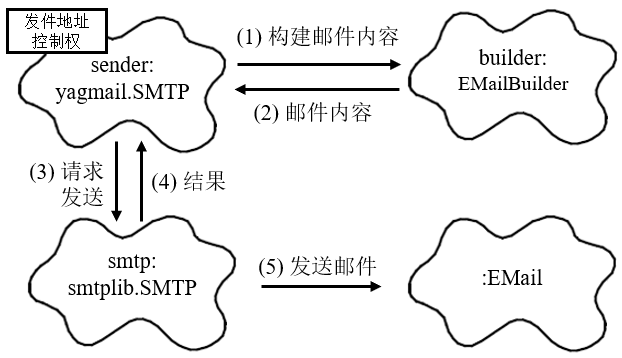
\includegraphics[width=0.65\textwidth]{figure/scene-2.png}
        \caption{Yagmail场景2:邮件的发送}
        \label{fig:scene-2}
    \end{figure}
    
\newpage
\section{Yagmail的可信性分析}

    本节,我们对Yagmail软件系统的可信性进行了分析评估。首先,我们总结了Yagmail在可信性方面应具备
    的诸项需求。然后,通过对Yagmail软件架构、调用路径、程序逻辑与源代码的分析,验证了Yagmail具体
    是如何满足、保障各项可信性需求的。最后,借助一些在软件可信性分析方面进行更具体的量化分析的
    方法,从定性走向定量,对Yagmail的可信性进行了进一步的度量。
    
    软件可信性是一个新鲜的概念。在对可信性进行具体分析之前,有必要适度明确可信性的概念。结合
    \cite{researchreview}和\cite{courseware}对软件可信性的定义,
    我们认为“可信性”指的是软件系统在实现既定功能时,
    行为和结果是可以预测的、可以控制的。即使是在受到各种外部干扰(特殊情况)时,也具备较高的
    容错性。为了提高软件的可信性,需要在可用性、功能、可靠性(容错)、安全性(机密性、完整性)、
    性能(响应时间、资源消耗)、维护代价等多方面共同优化。

\subsection{可信性需求}

    本小节,我们将对Yagmail在可信性方面应具备的基本需求进行列举说明,具体如下。

    1.(高可用性)当正确调用Yagmail发送邮件时,邮件发送的成功率要高。
    
    2.(高可用性)进行登录认证时,在信息输入正确的情况下,登陆成功率要高。
    
    3.(高容错性)当登陆或邮件发送失败时,需要给用户反馈,提示错误原因,并有相应的错误处理机制和记录。
    
    4.(高容错性)对用户填写的邮件地址,需要验证合法性。
    
    5.(高安全性)进行登录认证时,必须保证用户隐私信息不被泄露,
    
    6.(高安全性)邮件发送到指定的收件人,而不是第三方。
    
    7.(高安全性)邮件内容格式要保留完整。
    
    8.(性能)邮件发送的响应时间要快,资源占用要低。
    
    以上为Yagmail应满足的主要的可信性需求。

\subsection{可信性保障}

    本小节,我们将对Yagmail具体是如何满足、保障上一小节所提到的各项可信性需求,进行分析说明。
    在具体分析Yagmail的可信性实现之前,有必要对它的各组件的依赖关系进行说明。我们借助Pyan工具
    \cite{pyan}:一款针对Python语言的静态分析、组件/函数调用图
    以及“define-use”链路绘制工具,对Yagmail进行组件图分析绘制。绘制层级到组件级而非函数级,
    图中的箭头表示“use”关系,“define”关系不在图中体现。
    
    \begin{figure}[H]
        \centering
        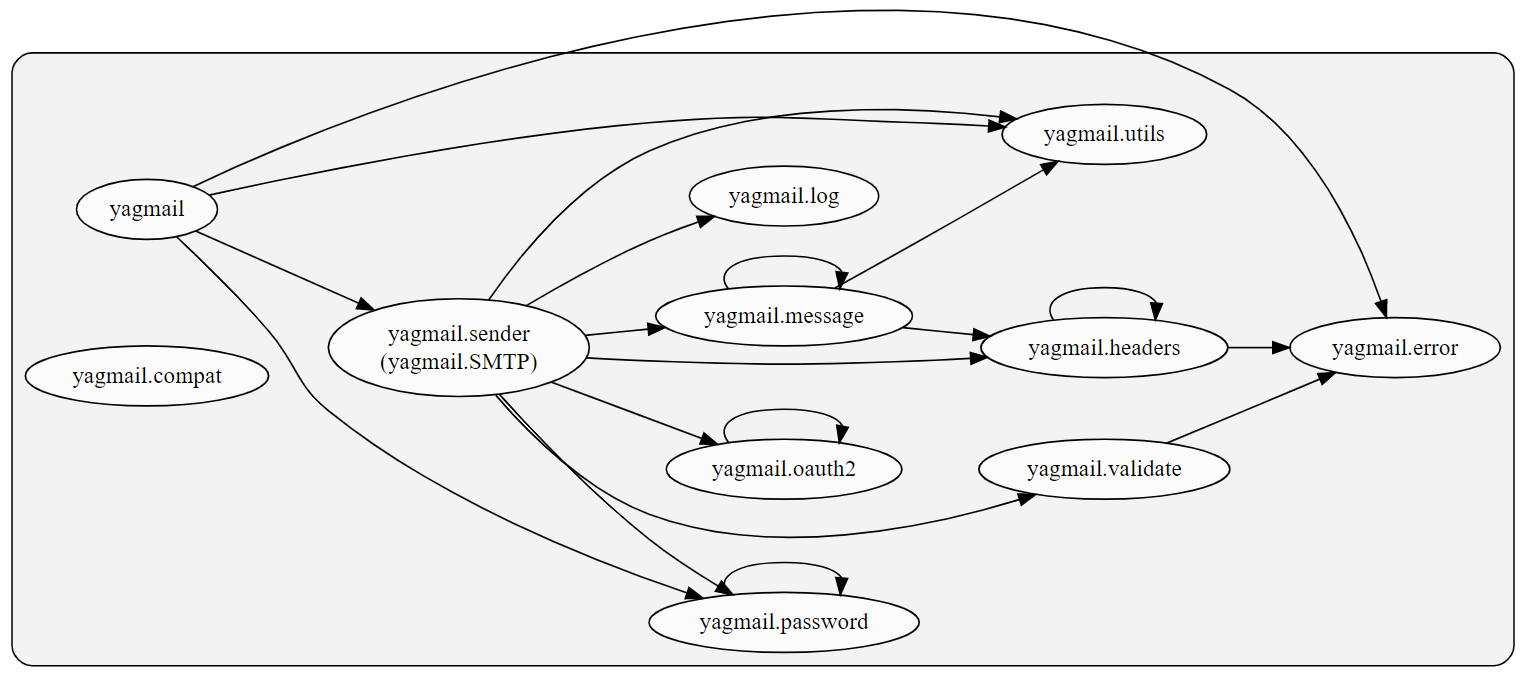
\includegraphics[width=0.99\textwidth]{figure/component-dep-graph.png}
        \caption{Yagmail的组件依赖图}
        \label{fig:component-dep-graph}
    \end{figure}
    
    \subsubsection{高可用性}
    
    为了对高可用性进行保障,在发送邮件的成功率方面,Yagmail第一次发送失败时,
    会再尝试两次间隔3、6秒的重新发送,以提高发送的成功率。
    如果仍然失败,则记录下来。从软件架构层面看,结合前文的开发视图,
    本部分职责由顶层组件yagmail.sender完成,相关代码如下:
    
    \begin{lstlisting} 
    while attempts < 3: # 最大尝试次数为3
        try:
            result = self.smtp.sendmail(self.user, recipients, msg_string)
            self.log.info("Message sent to %s", recipients)
            return result # 发送成功,直接返回
        except smtplib.SMTPServerDisconnected as e: # 发送出现异常
            self.log.error(e)
            attempts += 1
            time.sleep(attempts * 3) # 间隔一段时间重新发送
    self.unsent.append((recipients, msg_string)) # 仍然失败,保存相关信息
    \end{lstlisting}
    
    \subsubsection{高容错性}
    
    对用户填写的邮件地址,结合前文的开发视图,Yagmail的较低层次的yagmail.validate组件
    会使用基于RFC 2822标准构建的正则表达式,验证邮件地址的格式。如果不符合要求,
    则会报错提示不符合RFC 2822的标准。但无法验证该邮件地址是否为实际注册存在的邮件地址。
    
    \begin{lstlisting} 
    def validate_email_with_regex(email_address):
        if not re.match(VALID_ADDRESS_REGEXP, email_address): # 使用正则表达式验证
            emsg = 'Emailaddress "{}" is not valid according to RFC 2822 standards'.format(email_address)
            raise YagInvalidEmailAddress(emsg) # 发起异常
    \end{lstlisting}

    \subsubsection{高安全性}

    在登陆时,除了明文账号密码方式以外,Yagmail还提供更安全先进的OAuth验证方式,对GMail发件邮箱可使用Google授权口令授权,起到了保障用户邮箱、密码等隐私信息的作用
    另外,Yagmail还提供基于操作系统Keyring的认证方式,存储密码信息。具体做法是使用register方法,
    其内部调用keyring库,将相关隐私信息存入操作系统。
    以上这些在软件架构层面,结合前文绘制的开发视图和逻辑视图,主要由中间层次的发件地址权限控制
    类模块实现。它们利用了底层模块提供的功能,并对更高层次的模块给与权限与安全保障。
    
    \begin{figure}[H]
        \centering
        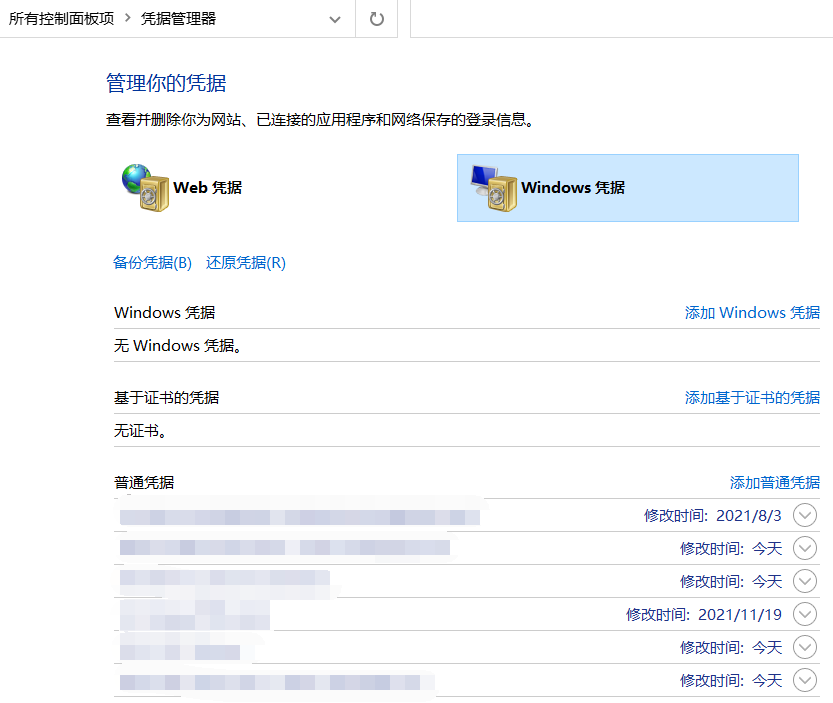
\includegraphics[width=0.65\textwidth]{figure/windows-keyring.png}
        \caption{Windows系统的Keyring服务:凭据管理器}
        \label{fig:windows-keyring}
    \end{figure}
    
    上述步骤的相关代码如下所示:
    \begin{lstlisting}
    yag = yagmail.SMTP("user@gmail.com", oauth2_file="~/oauth2_creds.json") # OAuth认证方式
    yagmail.register('myUsername', 'myPassword') # 登记Keyring信息
    keyring.set_password('yagmail', 'myUsername', 'myPassword') # 内部调用keyring库实现
    \end{lstlisting}
    
    \subsubsection{性能}
    
    为了提高Yagmail的整体性能,在执行时间方面,Yagmail的组件依赖关系简单,调用路径短,
    这使得执行的效率得到提高;在资源占用方面,Yagmail的依赖库绝大部分都是Python内部的标准库,
    整体库大小控制在了60KB左右,资源占用低,更易于集成到其他软件系统。对于Yagmail性能的测试,
    将在下一小节更具体地介绍。

\subsection{可信性度量}

    本小节,我们按照\cite{thebook}中提供的基于可靠概率法的可靠性度量方法,以及
    使用圈复杂度和扇入扇出度的可维护性度量方法,对Yagmail的可信性在这两个方面
    进行度量,以获得更细致的定量的分析结果;使用插桩(Stub)Mock法,对Yagmail进行了性能度量;
    按照\cite{opensource}提出的基于用户评价、迭代和缺陷跟踪的开源软件可信性评价方法,
    阐述了一种对Yagmail在用户侧的可信性进行度量的做法。在整体流程中,我们还借鉴了
    \cite{misc1}\cite{misc2}中的一些思路。

    \subsubsection{可靠性度量:使用可靠概率法}
    
    可靠概率RP的度量结果为一个实数值,用来表示软件系统正常运行时软件架构不会发生错误的概率。
    为简化分析,我们以分析Yagmail的场景视图的场景2:邮件的发送为例。在UML模型中,
    场景由UML顺序图表示。因此,首先将图8重绘为UML顺序图,如下图所示:
    
    \begin{figure}[H]
        \centering
        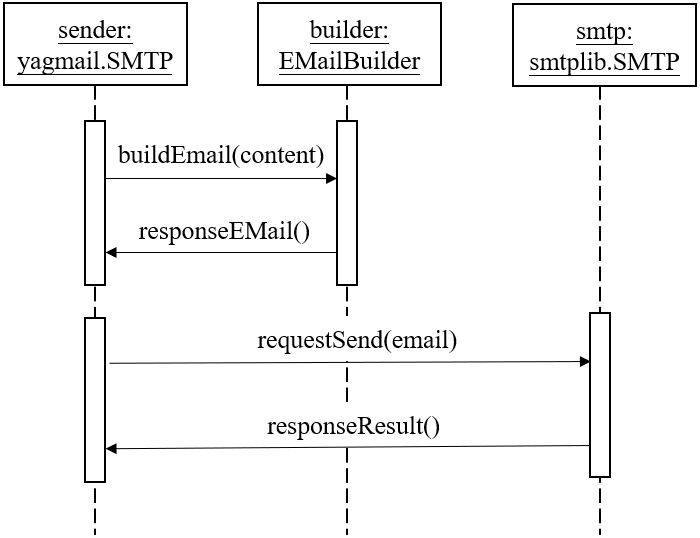
\includegraphics[width=0.6\textwidth]{figure/uml-seq.png}
        \caption{“场景2:邮件的发送”的UML顺序图}
        \label{fig:uml-seq}
    \end{figure}
    
    首先考虑组件对场景可靠性的影响。将所使用的的三个组件$i$和一次执行
    平均可能故障概率${\rm component}_i$列表如下:
    
    \begin{table}[H]
    \centering
    \caption{“场景2:邮件的发送”的组件平均可能故障概率}
    \label{tab:my-table}
    \begin{tabular}{l|l}
    \hline
    \textbf{组件$i$}          & \textbf{${\rm component}_i$} \\ \hline
    yagmail.SMTP & 0.5 \%                            \\ \hline
    EMailBuilder & 0.2 \%                            \\ \hline
    smtplib.SMTP & 0.1 \%                            \\ \hline
    \end{tabular}
    \end{table}
    
    对于组件smtplib.SMTP,由于其为Python语言标准库的一部分,故认为其故障概率很低,为0.1\%。
    对于Yagmail内部的组件,由于没有运行时的遥测(Telemetry)回传数据,我们依据先验知识对故障概率
    进行设定。EMailBuilder的职能相对简单,故赋较小的故障概率;yagmail.SMTP的工作内容较为复杂,
    外部调用多,故赋较大的故障概率。
    
    其次考虑连接件对场景可靠性的影响。由于对物理连接件,如网卡、电缆、光纤等硬件和介质的
    失败概率分析已超出对Yagmail的软件架构进行分析的范畴,故我们取物理连接件的失败概率
    ${\rm connector}_j=0$。
    
    综上,结合各组件在场景中的被调用次数$x_i$,我们可计算出该场景的可靠概率:
    
    \begin{equation}
    \begin{aligned}
        & {\rm ssp} = p_{\rm component} \times p_{\rm connector}\\
        & =\Pi_i(1-{\rm component}_i)^{x_i} \times 1\\
        & =(1-0.005)^2 \times (1-0.002)^1 \times (1-0.001)^1 \times 100\%\\
        & =98.7\%
    \end{aligned}
    \end{equation}

    可见,在当前的软件架构下,Yagmail有效控制了各组件的被调用次数,以达到对整体失败概率
    进行控制的效果,系统整体可靠概率高。

    \subsubsection{可维护性度量:使用圈复杂度和扇入扇出度}

    在软件架构度量和评估中,圈复杂度表示组件图中由模块依赖关系组成的依赖控制路径
    的数量;而扇入指的是直接调用该模块的上级模块的数量;扇出指的是该模块调用下级模块的
    数量。
    
    我们选择对Yagmail的核心组件:Yagmail.SMTP进行可维护性度量。结合图9绘制的各组件之间的
    依赖关系图,根据与Yagmail.SMTP相关的组件提取出来构成的子图,以及对源代码中import
    关系的分析,可得到如下表所示的数据:
    
    \begin{table}[H]
    \centering
    \caption{Yagmail可维护性度量数据}
    \label{tab:maintain-measure}
    \begin{tabular}{|l|l|l|l|}
    \hline
    \multicolumn{1}{|c|}{\textbf{项目}}                          & \multicolumn{1}{c|}{\textbf{符号}} & \multicolumn{1}{c|}{\textbf{值}} & \multicolumn{1}{c|}{\textbf{说明}}                                                                           \\ \hline
    \begin{tabular}[c]{@{}l@{}}组件图中所有外部组件\\ 的数目\end{tabular}   & $totalN$                         & 9                               & \begin{tabular}[c]{@{}l@{}}顶层包、log、message、oauth2、\\ password、utils、headers、\\ validate、error\end{tabular} \\ \hline
    \begin{tabular}[c]{@{}l@{}}组件图中所有外部组件\\ 的关联关系\end{tabular} & $totalE$                         & 15                              & \begin{tabular}[c]{@{}l@{}}不含组件内部的关联关系,即去\\ 掉内部关联边的总边数\end{tabular}                                        \\ \hline
    层数                                                         & $L$                              & 2                               & \begin{tabular}[c]{@{}l@{}}UML组件图数目,仅有compat组件\\ 游离在与yagmail.SMTP相关的子图外\end{tabular}                       \\ \hline
    该组件对其他组件的依赖                                                & $E$                              & 7                               & 出边数量                                                                                                       \\ \hline
    该组件提供的接口数                                                  & $W$                              & 2                               & -                                                                                                          \\ \hline
    其他组件对该组件的依赖                                                & $X$                              & 2                               & 仅顶层包中存在                                                                                                    \\ \hline
    \begin{tabular}[c]{@{}l@{}}该组件调用其他组件\\ 的接口数\end{tabular}   & $R$                              & 9                               & -                                                                                                          \\ \hline
    \end{tabular}
    \end{table}
    
    由上表列出的数据,代入相关公式,可计算出圈复杂度:
    
    \begin{equation}
    \begin{aligned}
        & {\rm CCN} = (totalE - totalN) + 2L\\
        & =(15 - 9) + 2 \times 2\\
        & =10
    \end{aligned}
    \end{equation}
    
    \noindent
    圈复杂度小于等于10,是一个较为适宜的值。
    
    同理可计算出扇入扇出度:
    
    \begin{equation}
    \begin{aligned}
        & {\rm FFC} = {\rm CCN} \times ((E+W)\times(X+R))^2\\
        & =10 \times ((7+2)\times(2+9))^2\\
        & =98010
    \end{aligned}
    \end{equation}
    
    \noindent
    其中扇入指标主要由$W$、$X$表现,扇出指标主要由$E$、$R$表现,可以看出,由于Yagmail.SMTP是一个
    偏顶层的模块(正如“图5:开发视图”所示),所以表现出扇出比较大的特性,符合优秀、典型的软件架构
    的特点。
    
    Yagmail在可维护性度量方面的优秀、典型的指标,恰说明了Yagmail的软件架构的优秀性。因为只有
    适当组织软件架构各层级、各模块之间的依赖、调用关系,才能获得好的圈复杂度和扇入扇出相关指标。
    
    \subsubsection{性能度量:使用插桩(Stub)Mock模拟法}

    在软件测试领域,代码插桩(Stub)技术是一种常用的测试辅助技术。它使得测试人员在对软件的一部分
    进行测试时,可以为依赖但还未完成的部分暂时用一段代码“占坑”,以临时切断这种依赖关系,使得测试
    得以继续。这种技术的一种实现是Mock模拟方法,即通过随机数据,模拟多种场景。该部分的实验代码在
    yagmail-stub-mock目录下。
    
    由于Yagmail的登陆和邮件发送功能的流程与邮件发送服务器强相关,而倘若构造一系列真实的邮件发送
    情景,实验成本较高,且大部分邮件服务提供商对此类通过脚本大规模发送邮件的行为,都有相应的
    风险控制策略,容易触发警报。因此,我们使用模拟数据接口对Yagmail的邮件发送功能(yagmail.SMTP.send)进行性能测试,以简化测试流程,规避上述问题。
    
    我们使用Mock技术,融入先验知识,模拟两部分内容:
    
    一是Yagmail与远端邮件发送服务器进行通讯时的时间消耗(往返时延)$RTT$,其模拟值为从正态分布
    $N(\mu, \sigma) = N(1.5, 0.5)$的采样,且要求
    $0 < RTT < 3$,单位为秒。这表示在邮件发送时网络通讯部分的耗时绝大部分落在1到2秒的范围内,
    最大不超过3秒,这符合现有主流个人邮件服务提供商侧的性能水平。对得到的$RTT$,在进行邮件发送时
    按该时间阻塞程序,以模拟Yagmail对服务器响应的等待。
    
    二是Yagmail在进行邮件发送时邮件发送服务器的发送成功概率。其生成方式为,当从均匀分布
    $U(0, 1)$上采样的一随机值$p > 0.5\%$时,为发送成功,即发送失败率约为$0.5\%$,
    这符合现有主流个人邮件服务提供商侧的成功率水平。当模拟发送失败时,即会触发Yagmail的高可用性
    重试逻辑。
    
    以模拟内容一为例,在完成代码Mock前后,代码的变异如下:
    
    \begin{lstlisting}
    # Mock前:需要与外部服务器联系
    result = self.smtp.sendmail(self.user, recipients, msg_string)
    
    # Mock后:切断了外部依赖
    waitTimeSec = randomInRangeGauss(0, 3, 1.5, 0.5)
    self.slpTimesTot += waitTimeSec # 记录总RTT
    time.sleep(waitTimeSec) # 模拟等待
    \end{lstlisting}
    
    固定仅需执行一次的登录操作的时间消耗为3秒,模拟发送500封邮件。测试过程中,Yagmail承受住
    了串行压力,面对发送失败的错误也没有发生崩溃。测试过程图、相关代码如下所示:
    
    \begin{figure}[H]
        \centering
        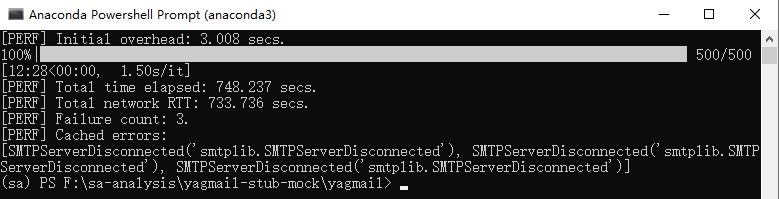
\includegraphics[width=0.8\textwidth]{figure/perf.png}
        \caption{邮件发送性能测试项目测试过程图}
        \label{fig:perf}
    \end{figure}
    
    \begin{lstlisting}
    # 求初始化时间开销
    tic = time.time(); smtp = yagmail.SMTP(user='MOCK'); toc = time.time() + LOGIN_TIME
    
    # 求模拟500封发送的时间开销
    tic = time.time()
    for i in tqdm(range(SEND_COUNT)):
        smtp.send()
    toc = time.time()
    \end{lstlisting}
    
    通过整理数据,可得到性能测试结果表如下:
    
    \begin{table}[H]
    \centering
    \caption{性能测试结果表}
    \label{tab:perf-result}
    \begin{tabular}{|l|l|cl}
    \hline
    \multicolumn{1}{|c|}{\textbf{项目}} & \multicolumn{1}{c|}{\textbf{耗时(秒)}}                               & \multicolumn{1}{c|}{\textbf{项目}} & \multicolumn{1}{c|}{\textbf{值}} \\ \hline
    初始化与登陆耗时                          & 3.008                                                             & \multicolumn{1}{l|}{邮件发送失败数}     & \multicolumn{1}{l|}{3}          \\ \hline
    Yagmail初始化耗时                      & 3.008-3=0.008                                                     & \multicolumn{1}{l|}{邮件发送成功率}     & \multicolumn{1}{l|}{99.4 \%}    \\ \hline
    邮件发送总耗时                           & 748.237                                                           & \multicolumn{1}{l|}{程序崩溃率}       & \multicolumn{1}{l|}{0}          \\ \hline
    总RTT                              & 733.736                                                           & \multicolumn{2}{c}{\multirow{3}{*}{(下空)}}                          \\ \cline{1-2}
    邮件发送Yagmail耗时                     & \begin{tabular}[c]{@{}l@{}}748.237-733.736\\ =14.501\end{tabular} & \multicolumn{2}{c}{}                                               \\ \cline{1-2}
    平均每封Yagmail耗时                     & 14.501/500=0.03                                                   & \multicolumn{2}{c}{}                                               \\ \cline{1-2}
    \end{tabular}
    \end{table}
    
    可见,略去与网络、服务商等外界因素相关的耗时,Yagmail在邮件发送上消耗的时间极少,整体性能
    很高,且在快速的同时,保持了较高的成功率。这样优秀的表现与Yagmail优秀的软件架构是分不开的。
    这验证了我们在3.2.4节的判断,并且我们将在第四节的实验中进一步分析、证明这一点。

    \subsubsection{开源软件用户侧可信性度量:基于用户评价、迭代和缺陷跟踪}

    通过文献阅读,我们从\cite{opensource}了解到,对于开源软件,
    可以通过爬取缺陷跟踪系统中的可信证据,
    对可信属性之间的联系进行分析,评价组件和开源软件自身在运行时的可信性。而Yagmail在GitHub平台
    开源的特点,使得它天生就具备Issues这一缺陷追踪渠道,且可从中获知用户评价数据;它还天生具有
    Pull Request这一迭代追踪渠道,可以了解各缺陷的迭代修复过程。这些数据让我们能够利用该文献中的
    方法,对Yagmail的用户侧可信性进行度量。
    
    由于该文献中提到的方法实现过程较为复杂,且所需数据需要爬取、仔细清洗后才可开始分析流程,因此
    本文此处仅做介绍提及。

\newpage
\section{实验:Yagmail软件架构的变异与对比}
    
    为了进一步说明Yagmail的软件架构设计对软件可信性的影响,本节将对Yagmail在软件架构进行一定
    的变异、修改,引入架构坏味道。接着,将前后版本的Yagmail进行对比,发现架构变异对软件可信性
    的负面作用。本部分实验的相关代码在yagmail-bad-smell目录下。
    
\subsection{实验实施}

    根据\cite{thebook}的叙述,软件架构层面的坏味道是一种设计级的坏味道,其抽象层次更高。
    本文对Yagmail
    变异出如下三个种类的架构坏味道:组件嫉妒(Component Envy)、
    过度分散的功能(Scattered Functionality)、模糊接口(Ambiguous Interface)。
    
    \textbf{为形成组件嫉妒},我们将验证登录环节的OAuth型验证方式的实现交由yagmail.SMTP内部实现,
    取消对yagmail.oauth2的导入。这样,增加了yagmail.SMTP组件的功能。
    
    \textbf{为变异出过度分散的功能},我们将验证邮件地址的合法性的yagmail.validate模块的核心功能
    validate\_email\_with\_regex复制一份到工具模块yagmail.utils中,因为该功能也符合
    工具功能或辅助功能的定义。但在yagmail.validate模块中的实现,该功能认为即使没有点号,
    邮件地址也可能是合法的,因为当用户是在某个局域网、使用自建DNS,或者修改了Hosts文件的情况下,
    上述邮件地址确实可能被解析。
    
    \textbf{为了引入模糊接口},我们允许用户在调用yagmail.SMTP模块的核心功能send发送邮件时,在
    “主题”(Subject)一项参数中填入数字值。如此,在确定邮件主题时,需要加一步对数据类型的
    判断,如果为数字值,需要先将其转换为字符串表示。该功能是有意义的,因为一些通知类或内部
    信息邮件的主题,可以用纯数字表示ID编号,以便归档。
    
    在完成上述变异流程后,我们使用与第三节类似的软件可信性的分析方式,对变异版本的Yagmail
    重复可信性分析,并进行对比。相关结果与分析于下一小节展示。

\subsection{结果与分析}
    
    在完成上一小节提到的变异修改后,yagmail.SMTP模块的内部调用链路图如下图所示(使用Pyan绘制):
    
    \begin{figure}[H]
        \centering
        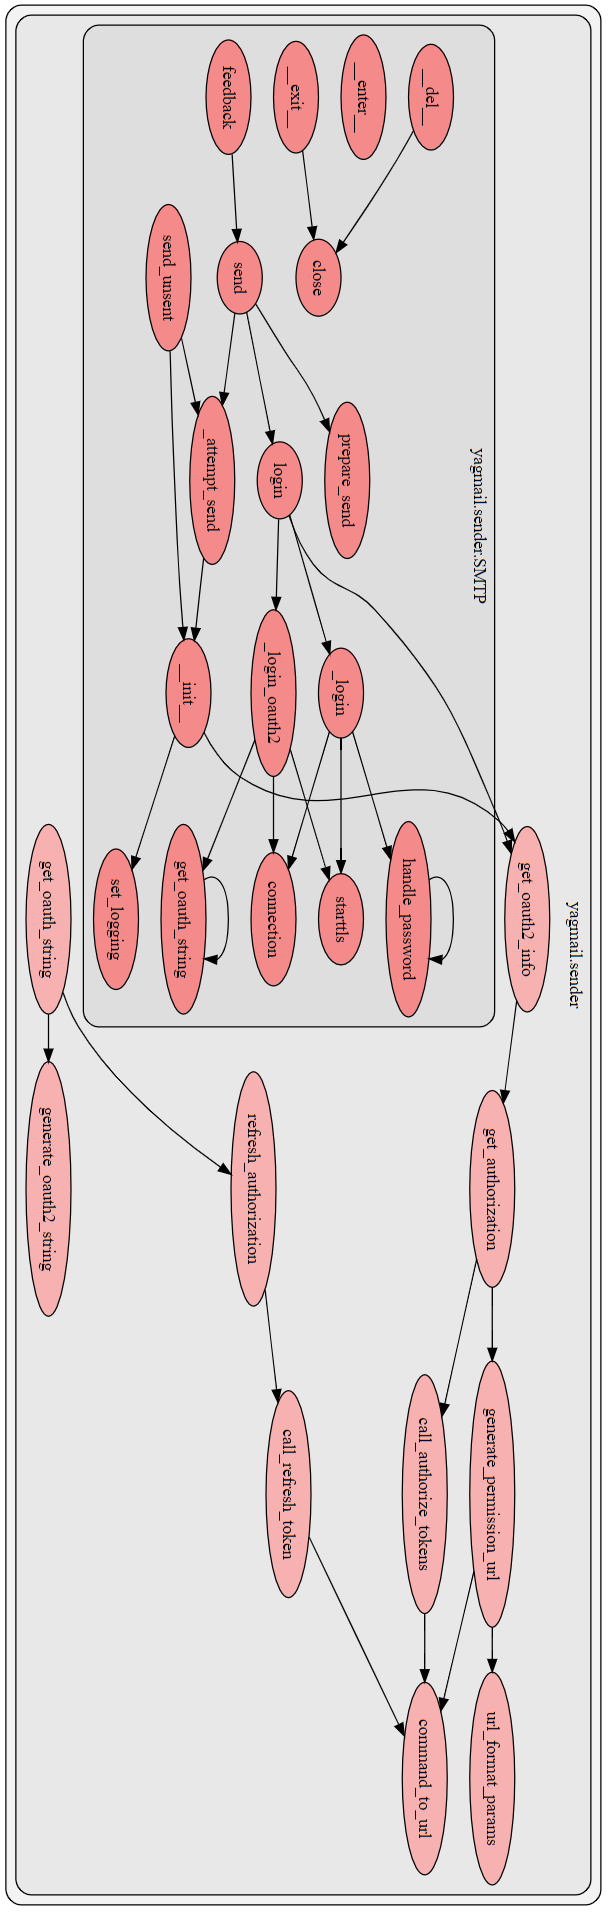
\includegraphics[height=0.95\textheight]{figure/changed-function-graph-only-sender.png}
        \caption{变异后的yagmail.SMTP模块的内部调用链路(经旋转以清晰展示)}
        \label{fig:changed-callgraph}
    \end{figure}

    \textbf{组件嫉妒}变异导致了函数调用路径的变化,OAuth认证不再需要涉及其他模块,这似乎降低了
    yagmail.SMTP
    组件的圈复杂度,但该架构违背了单一职责原则,内部调用链路复杂了许多,进一步地导致了组件的
    可测试性、可理解性和可复用性的降低:可理解性的降低体现在yagmail.SMTP模块既要负责邮件的发送,
    又要负责发件地址权限的控制,这导致
    “图5:开发视图”中的第3层和第5层混杂在一起,如下图所示。这破坏了分层结构,
    难以总结、理解该模块实现的功能;
    可复用性的降低体现在模块的体积更大,引入的成本更高,并且低可理解性也加大了引入的心智负担;
    可测试性的降低是因为模块级的测试失败时,需要更多的工作用来确定具体是哪些函数或者哪条调用
    链路产生的问题。
    
    \begin{figure}[H]
        \centering
        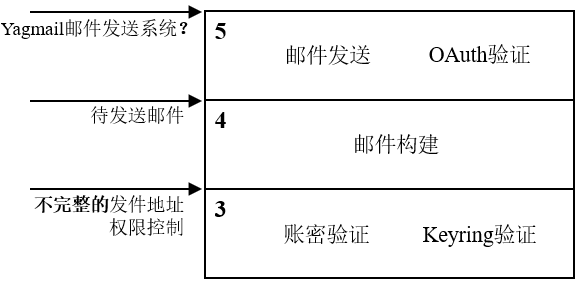
\includegraphics[width=0.6\textwidth]{figure/changed-dev-view.png}
        \caption{组件嫉妒下的开发视图变化}
        \label{fig:changed-dev-view}
    \end{figure}
    
    \textbf{过度分散的功能}使得组件的关注点不能很好地分离。关注点对组件的多重性,即组件对关注点的
    非正交性,会导致软件架构被破坏。对于需要使用同一功能的不同高层组件,可能会挑选不同的
    低层组件提供服务。则逻辑视图下连接关系将变多、变复杂,新加入的模块难以根据原有视图
    信息选择合适的低层模块。如下图所示,根据前文的“图3:逻辑视图”可知,yagmail.SMTP对基础设施
    类(如yagmail.util)和地址校验工具类(yagmail.validate)都有逻辑关联,此时其
    对validate\_email\_with\_regex功能的选择就出现二义。
    而在测试与维护方面,关注点向组件的不恰当对应还使得代价变大,需要对更多的组件进行测试与维护。

    \begin{figure}[H]
        \centering
        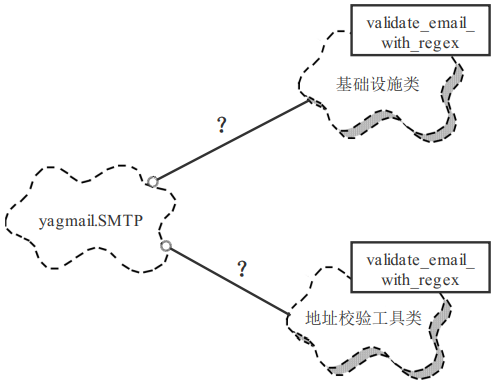
\includegraphics[width=0.6\textwidth]{figure/changed-log-view.png}
        \caption{过度分散的功能导致关注点难以分离}
        \label{fig:changed-log-view}
    \end{figure}
    
    \textbf{模糊接口}带来了应用性能的降低。程序需要对传入的数据的类型在运行时进行判断,
    必要时进行相应的转换。对于Python此类强类型动态类型语言,需要增加运行时类型判断与
    显式转换。倘若对于如
    C++这类静态类型语言,则还需要通过反射等运行时类型收集技术,妥善处理类型;对于JavaScript
    这类弱类型动态类型语言,类型转换过程经常成为安全漏洞的发生处。因此,无论是从运行的速度,
    还是运行的安全性来看,模糊接口对程序性能都有负面影响。
    
    综上所述,通过实验和后续的具体分析,我们可以得出引入架构坏味道对软件可信性存在负面影响,
    进一步说明了好的软件架构对软件可信性的重要性。
    
\newpage
\section{总结}

    在本课程作业中,我们首先通过FURPS+模型对Yagmail软件系统进行了多方面的需求分析说明,以对
    该软件系统的整体功能形成认识与把握。接着,我们应用Kruchten的“4+1”视图模型,对Yagmail软件
    系统的软件架构进行了多角度的观察与分析。
    
    在第三节,我们进一步应用从源码和架构层面的定性分析,
    以及基于度量的分析方式,对我们提出的Yagmail应具备的数项可信性需求的具体保障方式以及
    保障效果进行了分析说明。在第四节,我们则通过引入软件架构坏味道,对Yagmail的软件架构进行
    变异,以及可信性方面的对比分析。实验和分析表明,Yagmail对软件的可信性进行了行之有效的
    保障工作,整体可信性高,特别是软件架构的设计,对可信性起到了重要作用。在对软件架构进行
    负面的变异后,软件的可信性确实发生了降低,这更说明了好的软件架构对软件可信性的重要性。

    通过本次实验,我们对课堂所学知识有了更深入的消化吸收,并进行了实操应用。
    特别是通过对Yagmail软件功能、结构和使用的分析,对需求的FURPS+分析模型,以及软件架构
    的“4+1”视图模型的含义有了深入的了解,让之后的应用也更加得心应手。而在后面关于可信性
    的分析实验中,我们深刻体会到了软件可信性的重要性,以及好的软件架构对可信性的关键性,
    这将极大地指导我们日后的软件开发工作。
    
    
\begin{thebibliography}{99}
\setlength{\itemsep}{-1.5mm}
\addcontentsline{toc}{section}{参考资料}
\bibitem{yagmail} kootenpv. Yagmail [CP/OL]. 2021. https://github.com/kootenpv/yagmail.
\bibitem{furps} Grady Robert, Caswell Deborah. Software Metrics: Establishing a Company-wide Program [M]. Prentice Hall. 1987.
\bibitem{fourplusone} Philippe Kruchten. Architectural Blueprints—The “4+1” View Model of Software Architecture [J]. IEEE Software. 1995.
\bibitem{researchreview} 刘克. “可信软件基础研究”重大研究计划综述 [J]. 中国科学基金. 2008..
\bibitem{thebook} 李必信, 廖力, 王璐璐~等. 《软件架构理论与实践》 [M]. 机械工业出版社. 2019.
\bibitem{courseware} 李必信. 《软件开发方法与技术》课程课件 [EB/OL]. 2021. (内部资料).
\bibitem{pyan} Technologicat. Pyan [CP/OL]. 2021. https://github.com/Technologicat/pyan.
\bibitem{opensource} 孙晶, 刘丽丽. 开源软件可信性评价方法 [J]. 计算机工程与设计. 2017.
\bibitem{misc1} 吴晓娜, 李必信, 刘翠翠~等. 基于多维质量属性偏好的可信服务选择 [J]. 计算机应用与软件. 2012.
\bibitem{misc2} 王德鑫, 王青, 贺\hbox{\scalebox{0.6}[1]{吉}\kern-.2em\scalebox{0.6}[1]{力}}.  基于证据的软件过程可信度模型及评估方法 [J]. 软件学报. 2017.

\end{thebibliography}

\end{document}
